\documentclass[xetex,mathserif,serif]{beamer}
\usepackage{polyglossia}
\setdefaultlanguage[babelshorthands=true]{russian}
\usepackage{minted}
\usepackage{tabu}

\useoutertheme{infolines}

\usepackage{fontspec}
\setmainfont{FreeSans}
\newfontfamily{\russianfonttt}{FreeSans}

\definecolor{links}{HTML}{2A1B81}
\hypersetup{colorlinks,linkcolor=,urlcolor=links}

\tabulinesep=0.7mm

\newcommand{\attribution}[1] {
	\vspace{-5mm}\begin{flushright}\begin{scriptsize}\textcolor{gray}{\textcopyright\, #1}\end{scriptsize}\end{flushright}
}

\title{Архитектурная документация}
\subtitle{Design Documents}
\author[Юрий Литвинов]{Юрий Литвинов \newline \textcolor{gray}{\small\texttt{yurii.litvinov@gmail.com}}}

\date{18.03.2020г}

\begin{document}
	
	\frame{\titlepage}

	\begin{frame}
		\frametitle{Design Document, что это и зачем}
		\begin{itemize}
			\item Основной продукт работы архитектора
			\item Представляет и объясняет основные принятые архитектурные решения
			\begin{itemize}
				\item НЕ набор UML-диаграмм
			\end{itemize}
			\item Решение проблемы ``Architecture By Implication''
			\item Наличие хорошего диздока может сократить затраты на кодирование 
			\begin{itemize}
				\item в разы
			\end{itemize}
		\end{itemize}
	\end{frame}

	\begin{frame}
		\frametitle{Design Document, что это и зачем}
		\begin{itemize}
			\item В индустриальной практике он часто неформально, но обязательно присутствует --- как правило, это набор вики-страниц, иногда встречаются формальные документы
			\item Чеклист, позволяющий проверить, что обо всём подумали и всё служит какой-то осмысленной цели
			\item Не путать с Game Design Document (хотя он служит тем же целям и очень похож по структуре)
		\end{itemize}
	\end{frame}

	\begin{frame}
		\frametitle{Как писать}
		\begin{itemize}
			\item Достаточно подробно, чтобы при программировании не требовалось принимать важных архитектурных решений
			\item Разные \textit{точки зрения}, предназначенные для разных аудиторий
			\begin{itemize}
				\item Даже для одной целевой аудитории используется несколько точек зрения, например, статическая структура, поведение, схема БД и требования
			\end{itemize}
			\item Рекомендуется использовать диаграммы для иллюстрации архитектуры
		\end{itemize}
	\end{frame}

	\begin{frame}
		\frametitle{Как писать}
		\begin{itemize}
			\item Должен документировать не только принятые решения, но и:
			\begin{itemize}
				\item Альтернативы
				\begin{itemize}
					\item Чётко формулировать, что в итоге решили
				\end{itemize}
				\item Преимущества принятого решения
				\item Риски
				\item Связь с требованиями
			\end{itemize}
			\item Должны быть \textit{полнота} и \textit{консистентность}
			\item Стандарты IEEE 1016-2009 и ISO/IEC/IEEE 42010:2011
		\end{itemize}
	\end{frame}

	\begin{frame}
		\frametitle{Типичное содержание документа}
		\begin{itemize}
			\item Различная служебная информация
			\item Общие сведения о системе (несколько абзацев)
			\begin{itemize}
				\item Назначение
				\item Границы системы (Scope)
				\item Контекст, в котором существует система
			\end{itemize}
			\item Architectural drivers
		\end{itemize}
	\end{frame}

	\begin{frame}
		\frametitle{Architectural drivers}
		\begin{itemize}
			\item Architectural drivers --- ключевые требования, определяющие архитектуру
			\item Бывают:
			\begin{itemize}
				\item Технические ограничения
				\item Бизнес-ограничения
				\item Качественные характеристики системы
				\begin{itemize}
					\item Сопровождаемость, расширяемость и т.д.
					\item Масштабируемость, производительность
					\item Безопасность
				\end{itemize}
				\item Ключевые функциональные требования
			\end{itemize}
		\end{itemize}
	\end{frame}

	\begin{frame}
		\frametitle{Типичное содержание документа}
		\begin{itemize}
			\item Views (каждый из которых --- экземпляр Viewpoint-а)
			\begin{itemize}
				\item Требования, роли и случаи использования
				\item Структура системы
				\item Поведение системы
				\item Структура данных
				\item ...
			\end{itemize}
			\item Причины принятых решений, за/против
			\begin{itemize}
				\item Эта информация обычно приводится и во viewpoint-ах, тут summary
			\end{itemize}
		\end{itemize}
	\end{frame}

	\begin{frame}
		\frametitle{IEEE 1016, концепции документа}
		\begin{center}
			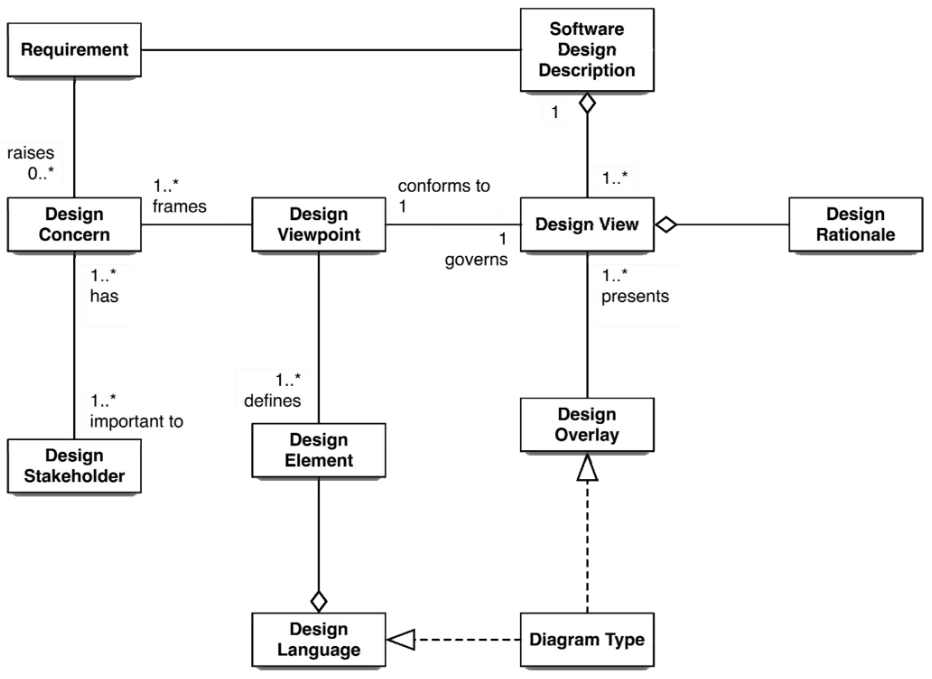
\includegraphics[width=0.8\textwidth]{ieee1016Concepts.png}
		\end{center}
	\end{frame}

	\begin{frame}
		\frametitle{IEEE 1016, элементы архитектуры}
		\begin{center}
			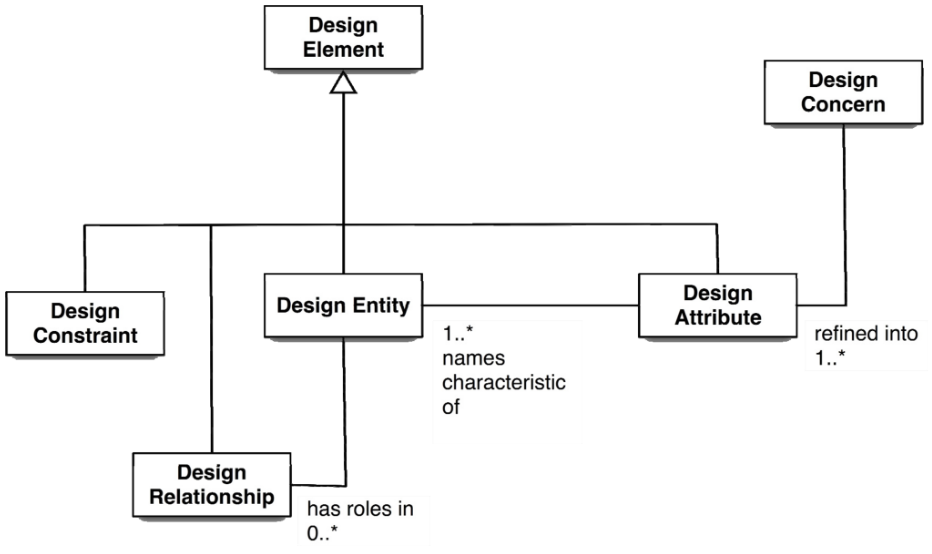
\includegraphics[width=0.8\textwidth]{ieee1016ArchitectureElements.png}
		\end{center}
	\end{frame}

	\begin{frame}
		\frametitle{IEEE 1016, точки зрения}
		\begin{itemize}
			\item Всего выделено 12 точек зрения
			\begin{itemize}
				\item Контекст
				\item Композиция
				\item Логическая структура
				\item Зависимости
				\item Информационная структура
				\item Использование шаблонов
				\item Интерфейсы
				\item Структура системы
				\item Взаимодействия
				\item Динамика состояний
				\item Алгоритмы
				\item Ресурсы
			\end{itemize}
			\item Все точки зрения в документе не обязательны
			\begin{itemize}
				\item Тем не менее, есть требование полноты
			\end{itemize}
			\item Есть ещё overlays --- виды с дополнительной информацией
		\end{itemize}
	\end{frame}

	\begin{frame}
		\frametitle{Контекст системы}
		\begin{itemize}
			\item Назначение --- описывает, что система должна делать, фиксирует окружение системы. Состоит из сервисов и акторов, которые могут быть связаны информационными потоками. Система представляет собой ``чёрный ящик''
			\begin{itemize}
				\item Может быть определён Deployment overlay
				\begin{itemize}
					\item Может быть отдельным видом, если аппаратное обеспечение --- часть разработки
				\end{itemize}
			\end{itemize}
			\item Соображения --- функциональные требования, роли, границы системы
			\begin{itemize}
				\item Корень иерархии уточняющих дизайн системы видов, стартовая точка при проектировании системы
			\end{itemize}
			\item Типичные языки --- диаграмма активностей UML, IDEF0 (SADT)
		\end{itemize}
	\end{frame}

	\begin{frame}
		\frametitle{Композиция}
		\begin{itemize}
			\item Назначение --- на самом деле, ``декомпозиция'', описывает крупные части системы и их предназначение
			\item Соображения --- локализация и распределение функциональности системы по её структурным элементам, impact analysis, переиспользование (в том числе, покупка компонентов), оценка, планирование, управление проектом, инструментальная поддержка (репозитории, трекер и т.д.)
			\item Типичные языки --- диаграммы компонентов UML, IDEF0
		\end{itemize}
	\end{frame}

	\begin{frame}
		\frametitle{Логическая структура}
		\begin{itemize}
			\item Назначение --- структура системы в терминах классов, интерфейсов и отношений между ними
			\begin{itemize}
				\item Используются также примеры экземпляров классов для пояснения решений
			\end{itemize}
			\item Соображения --- разработка и переиспользование
			\begin{itemize}
				\item Разделение на то, что можно взять и приспособить, и то, что придётся написать
			\end{itemize}
			\item Типичные языки --- диаграммы классов UML, диаграммы объектов UML
		\end{itemize}
	\end{frame}

	\begin{frame}
		\frametitle{Зависимости}
		\begin{itemize}
			\item Назначение --- определяет связи по данным между элементами
			\begin{itemize}
				\item Разделяемая между элементами информация, порядок выполнения и т.д.
			\end{itemize}
			\item Соображения --- анализ изменений, идентификация узких мест производительности, планирование, интеграционное тестирование
			\item Типичные языки --- диаграммы компонентов UML, диаграммы пакетов UML
		\end{itemize}
	\end{frame}

	\begin{frame}
		\frametitle{Информационная структура}
		\begin{itemize}
			\item Назначение --- определяет персистентные данные в системе
			\item Соображения --- информация, которую требуется хранить, схема БД, доступ к данным
			\item Типичные языки --- диаграммы классов UML, IDEF1x, ER, ORM
		\end{itemize}
	\end{frame}

	\begin{frame}
		\frametitle{ER, нотация Чена}
		\begin{center}
			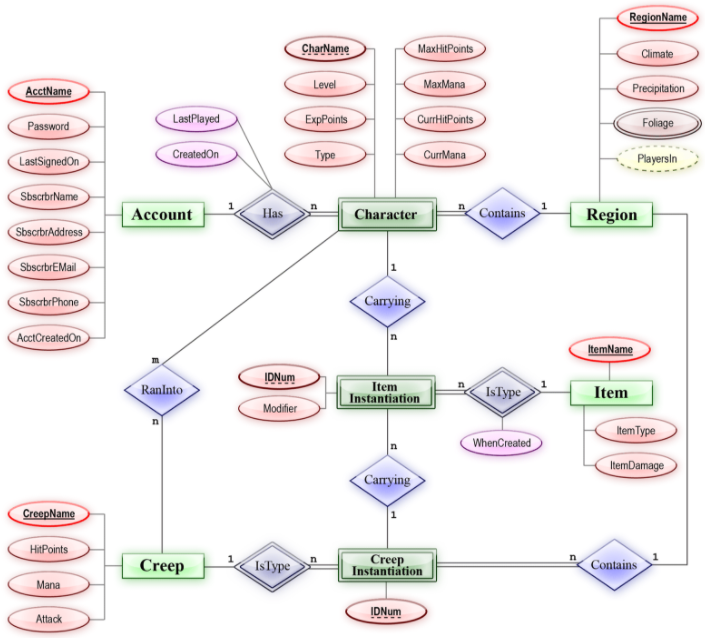
\includegraphics[width=0.6\textwidth]{erChenNotation.png}
			\attribution{https://ru.wikipedia.org}
		\end{center}
	\end{frame}

	\begin{frame}
		\frametitle{ER, нотация ``вороньей лапки''}
		\begin{center}
			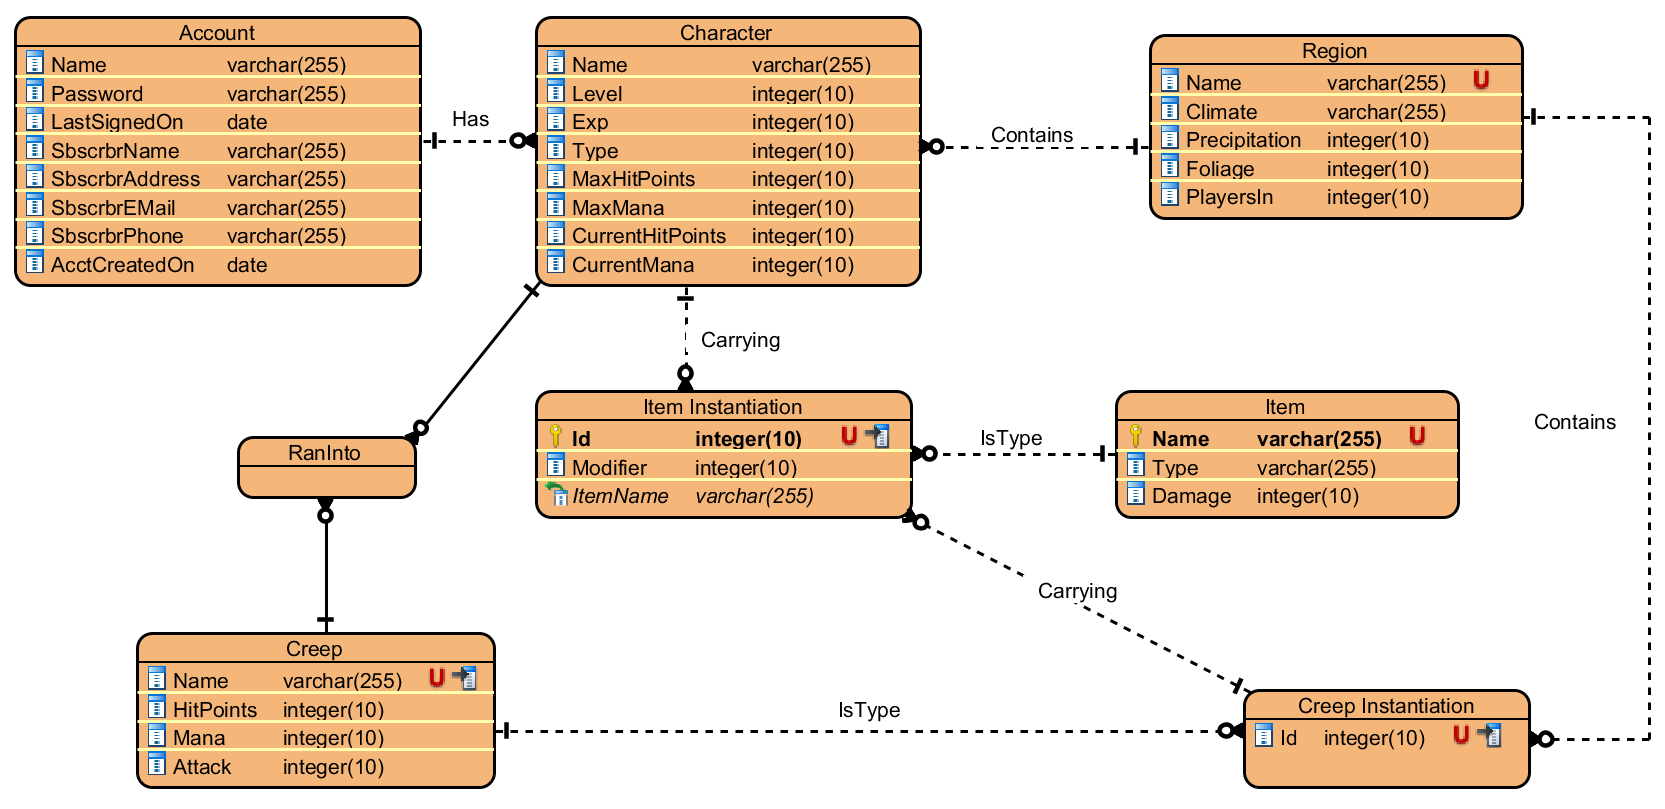
\includegraphics[width=0.9\textwidth]{erCrowsFoot.png}
		\end{center}
	\end{frame}

	\begin{frame}
		\frametitle{ORM, пример диаграммы}
		\begin{center}
			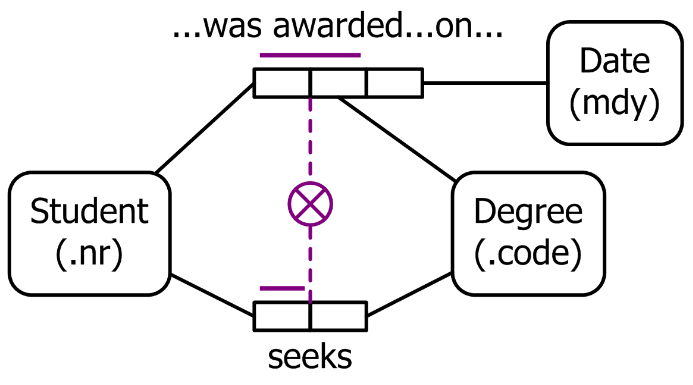
\includegraphics[width=0.6\textwidth]{orm.png}
		\end{center}
	\end{frame}

	\begin{frame}
		\frametitle{Использование шаблонов}
		\begin{itemize}
			\item Назначение --- документирование использования локальных паттернов проектирования
			\item Соображения --- переиспользование на уровне идей и архитектурных стилей
			\item Типичные языки --- диаграммы классов UML, диаграммы пакетов UML, диаграммы коллабораций UML
		\end{itemize}
	\end{frame}

	\begin{frame}
		\frametitle{Интерфейсы}
		\begin{itemize}
			\item Назначение --- специфицирует информацию о внешних и внутренних интерфейсах, не прописанную явно в требованиях
			\begin{itemize}
				\item Пользовательский интерфейс рассматривается отдельным видом в рамках этой точки зрения
			\end{itemize}
			\item Соображения --- договорённости о конкретных схемах взаимодействия компонентов, позволяющие разрабатывать и тестировать их независимо
			\item Типичные языки --- IDL, диаграммы компонентов UML, макеты пользовательского интерфейса, неформальные описания сценариев использования
		\end{itemize}
	\end{frame}

	\begin{frame}
		\frametitle{Структура системы}
		\begin{itemize}
			\item Назначение --- рекурсивное описание внутренней структуры компонентов системы
			\item Соображения --- структура системы, переиспользование
			\item Типичные языки --- диаграммы композитных структур UML, диаграммы классов UML, диаграммы пакетов UML
		\end{itemize}
	\end{frame}

	\begin{frame}
		\frametitle{Взаимодействия}
		\begin{itemize}
			\item Назначение --- описывает взаимодействие между сущностями: почему когда, как и на каком уровне выполняется взаимодействие
			\item Соображения --- распределение ответственностей между участниками взаимодействия, определение протоколов взаимодействия
			\item Типичные языки --- диаграммы композитных структур UML, диаграммы взаимодействия UML, диаграммы последовательностей UML
		\end{itemize}
	\end{frame}

	\begin{frame}
		\frametitle{Динамика состояний}
		\begin{itemize}
			\item Назначение --- описание состояний и правил переходов между состояниями в реактивных системах
			\item Соображения --- поведение системы, включая внутренние состояния, события и логику переходов
			\item Типичные языки --- диаграммы конечных автоматов UML, диаграммы Харела, сети Петри
		\end{itemize}
	\end{frame}

	\begin{frame}
		\frametitle{Сети Петри, пример}
		\begin{center}
			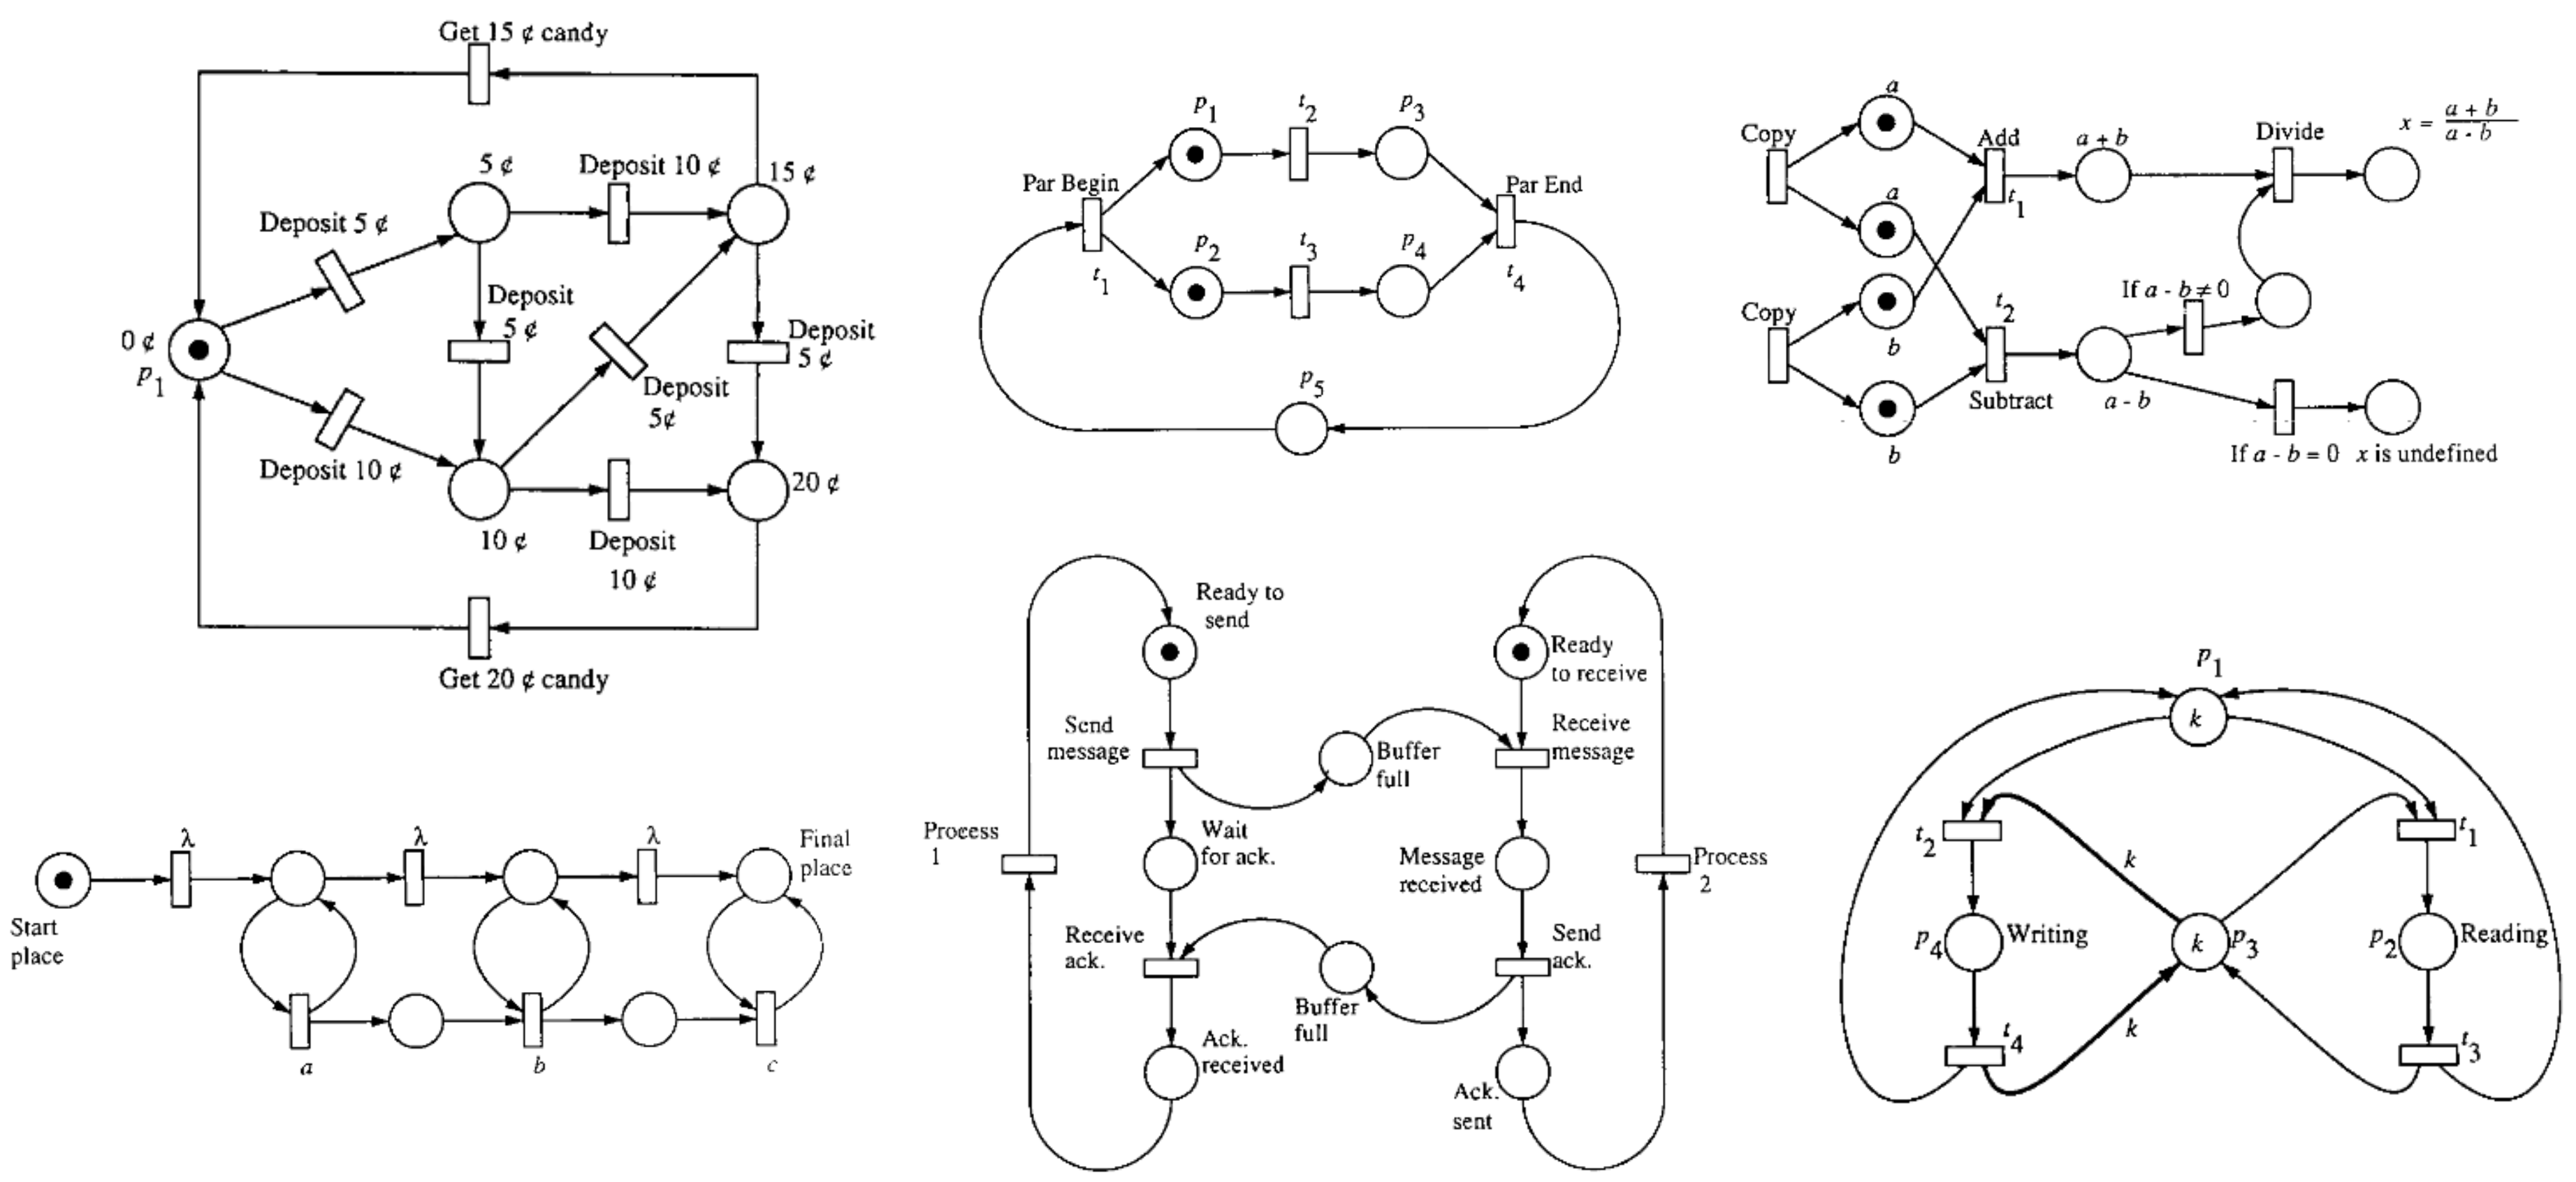
\includegraphics[width=\textwidth]{petriNet.png}
			\attribution{Murata Tadao. Petri nets: Properties, analysis and applications}
		\end{center}
	\end{frame}

	\begin{frame}
		\frametitle{Алгоритмы}
		\begin{itemize}
			\item Назначение --- описывает в деталях поведение каждой сущности, логику работы методов
			\item Соображения --- анализ эффективности работы программы, реализация, юнит-тестирование
			\item Типичные языки --- диаграммы активностей UML, псевдокод, настоящие языки программирования
		\end{itemize}
	\end{frame}

	\begin{frame}
		\frametitle{Ресурсы}
		\begin{itemize}
			\item Назначение --- описывает использование внешних ресурсов (как правило, аппаратных или третьесторонних сервисов)
			\item Соображения --- эффективность работы программы, доступность и эффективность использования ресурсов
			\item Типичные языки --- диаграммы развёртывания UML, диаграммы классов UML, OCL
		\end{itemize}
	\end{frame}

	\begin{frame}
		\frametitle{Примеры}
		\begin{itemize}
			\item Формальные документы:
			\begin{itemize}
				\item \url{http://robotics.ee.uwa.edu.au/courses/design/examples/example_design.pdf}
				\item \url{https://arxiv.org/ftp/arxiv/papers/1005/1005.0595.pdf}
			\end{itemize}
			\item Неформальные документы:
			\begin{itemize}
				\item \url{https://github.com/aspnet/EntityFramework/wiki/Design-Documents}
				\item \url{https://github.com/golang/proposal}
			\end{itemize}
		\end{itemize}
	\end{frame}

	\begin{frame}
		\frametitle{Домашнее задание: Roguelike}
		\begin{itemize}
			\item Жанр компьютерных игр, назван в честь игры Rogue, 1980 года выхода
			\item Характеризуется:
			\begin{itemize}
				\item Простой тайловой или консольной графикой
				\item Активным использованием случайной генерации
				\item Перманентной смертью персонажа и невозможностью загрузить предыдущее сохранение
				\item Чрезвычайно развитым набором игровых правил
				\item Высокой свободой действий персонажа (``игры-песочницы'')
			\end{itemize}
			\item Примеры:
			\begin{itemize}
				\item \url{https://en.wikipedia.org/wiki/NetHack}
				\item \url{https://en.wikipedia.org/wiki/Angband_(video_game)}
				\item \url{https://en.wikipedia.org/wiki/Ancient_Domains_of_Mystery}
			\end{itemize}
		\end{itemize}
	\end{frame}

	\begin{frame}
		\frametitle{Функциональные требования}
		\begin{itemize}
			\item Персонаж игрока, способный перемещаться по карте, управляемый с клавиатуры
			\begin{itemize}
				\item Карта обычно генерируется, но для некоторых уровней грузится из файла
				\item Характеристики --- здоровье, сила атаки и т.д.
				\item Экспа и уровни персонажа, с ростом уровня повышаются характеристики
			\end{itemize}
			\item Инвентарь персонажа, включающий элементы, влияющие на его характеристики, которые можно надеть и снять
			\item Несколько разных видов мобов, способных перемещаться по карте
			\item Боевая система --- движущиеся объекты, пытающиеся занять одну клетку карты, атакуют друг друга
		\end{itemize}
	\end{frame}

	\begin{frame}
		\frametitle{Домашнее задание}
		Разделиться на команды по три человека и написать архитектурное описание Roguelike
		\begin{itemize}
			\item Общие сведения о системе
			\item Architectural drivers
			\item Роли и случаи использования
			\begin{itemize}
				\item Описание типичного пользователя, как было в курсе по SE
			\end{itemize}
			\item Композиция (диаграмма компонентов)
			\item Логическая структура (диаграмма классов)
			\item Взаимодействия и состояния (диаграммы последовательностей и конечных автоматов)
			\item Всем диаграммам нужны словесные пояснения
			\item Это должен быть один документ (возможно, со ссылками на диаграммы)
		\end{itemize}
	\end{frame}

\end{document}